XMME (X-Machines Modelling Editor) provides the functionality of
designing and implementing agent specification and behavior. It is a
GUI application and the XMML (X-Machines Markup Language) provides the
underlying modeling schema.

In particular, XMME helps its user to visually edit an XMML formatted
file. XMML is a highly verbose and partially untyped data
specification language based on XML format. This sort of nature makes
it relatively difficult to edit individual XML files to describe
agents' specification and behavior which are very sophisticated in so
far that the agents have internal variable and external message
dependencies. Furthermore, the nested model fascility of XMML
specification makes it virtually unmanageable if it comes to large
models.

The XMME wraps the XMML specification and functionality by means of
nested data models. In its runtime, all the decoupled XMML files and
XMML nodes are managed by the application so that the model
specification remains consistent over time. By doing this, XMME does
not limit the XMML capabilities which allow to represent sophisticated
agent models, on the contrary, it helps modeler to deal with the
technical details and internal model specification consistency.

\bigskip

XMME is a free and open source software application which is developed
using C++ and Trolltech/QT development framework. The development idea
is based on content-presentation seperation, ie. the model internals
are controlled by a seperate routine which is a software library
called \texttt{libxmm2}. \texttt{libxmm2} provides the model whereas
XMME presents it to the user. At the same time, it passes all the user
input to the \texttt{libxmm2}. \texttt{libxmm2} is written purely in
C++ and core QT library which means that it can be used by any other
software routine, such as web server applications, command line
programs etc. During the EURACE software toolkit development phase,
developers have made extensive use of this library with
fast-prototyping principles. Beyond \texttt{libxmm2}, XMME uses QT's
model-view classes, which makes it easy to align to XMML while new
functionalities added to XMML specification.

Both XMME and and \texttt{libxmm2} are cross-platform applications. So
far, it has been ported to Microsoft Windows, GNU/Linux and MacOSX
operating systems.

\bigskip

XMME GUI design is based on two panes. Left pane provides a
hierarchical tree-view widget where all the XMML nodes are
represented. The right hand pane allows the user to edit available
nodes in detail.

A screenshot is provided below on Table \ref{xmmescreen}

\begin{figure}
  \centering
  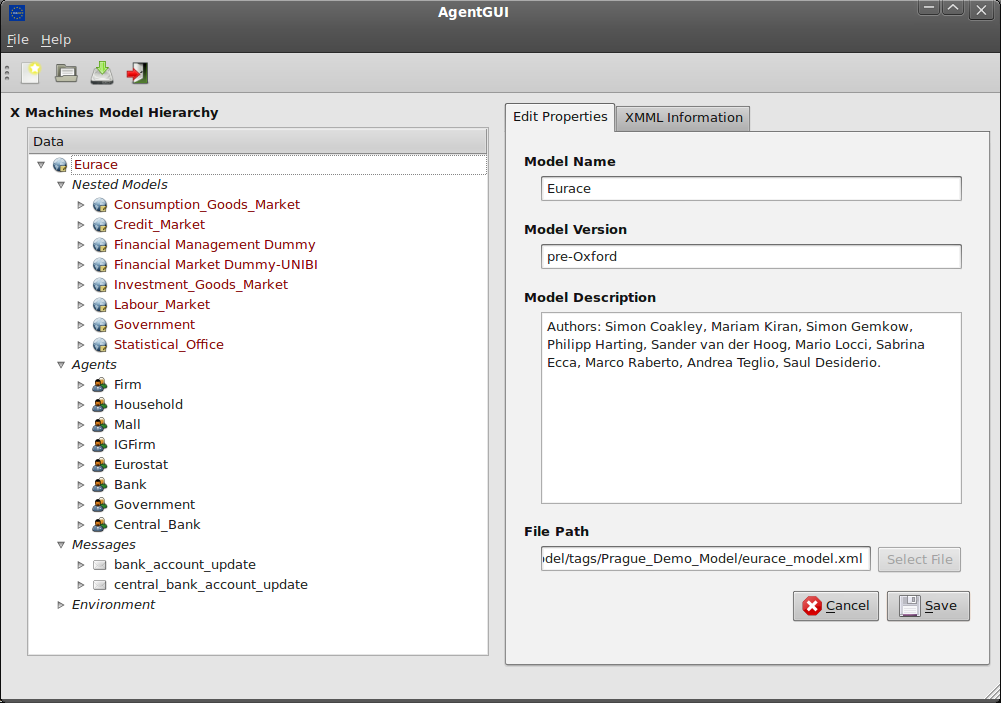
\includegraphics[width=14cm]{screenshots/xmmescreenshot.png}
  \caption{XMME (AgentGUI) Screenshot}
  \label{xmmescreen}
\end{figure}